\vspace{-0.5cm}
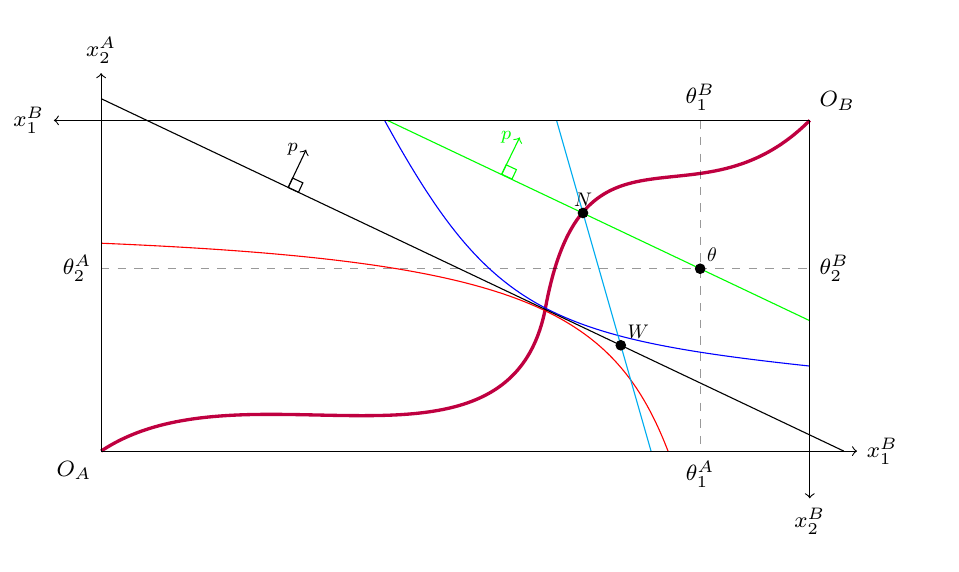
\begin{tikzpicture}[scale=1.2]
	\hspace{-0.3cm}
	% Curva de contrato 5.2,2
		\draw  [purple, very thick] (0.5,0.5) ..controls (2,1.5) and (4.8,0) .. (5.2,2) ..controls (5.6,4.2) and (6.8,2.8) .. (8,4);
		
	% Intersección de una dotación
		% Oferta: \theta
			\draw[dashed, opacity=0.4] (6.84,4) node [above, opacity=1] {\footnotesize $\theta_{1}^{B}$} -- (6.84,0.5) node [below, opacity=1] {\footnotesize $\theta_{1}^{A}$};
			\draw[dashed, opacity=0.4] (0.5,2.43)  node [left, opacity=1] {\footnotesize $\theta_{2}^{A}$} -- (8,2.43) node [right, opacity=1] {\footnotesize $\theta_{2}^{B}$};
	
	% Curvas de indiferencia
		\draw [blue] (3.5,4) .. controls (4.6,2) and (5.2,1.7) .. (8,1.4);
		\draw [red] (0.5,2.7) .. controls (4.915,2.515) and (5.915,2.015) .. (6.5,0.5);
	
	% Flecha y rectángulo
		\draw [->, green] (4.74,3.43) -- (4.93,3.82) node [left, scale = 0.3mm] {\footnotesize $p$};
		\draw [green, rotate around={-25:(4.74,3.43)}] (4.74,3.43) rectangle (4.86,3.54);
		
	% Recta presupuestaria
		\draw (0.5,4.23) -- (8.36,0.5);
		\draw [cyan](5.32,4) -- (6.32,0.5);
		\draw [green](3.53,4) -- (8,1.88);
	
	% Flecha y rectángulo
		\draw [->] (2.48,3.29) -- (2.67,3.69) node [left, scale = 0.3mm] {\footnotesize $p$};
		\draw [rotate around={-25:(2.48,3.29)}] (2.48,3.29) rectangle (2.6, 3.4);
	
	% Puntos
		\draw[black, fill=black] (5.6,3.02) circle[radius=0.05] node [above, scale=0.25mm] {$N$};
		\draw[black, fill=black] (6,1.62) circle[radius=0.05] node [above right, scale=0.25mm] {$W$};
		\draw[black, fill=black] (6.84,2.43) circle[radius=0.05] node [above right, scale=0.25mm] {$\theta$};
	
	% Formación de la caja
		% Consumidor A
			\draw[->] (0.5,0.5) node[align=center, below left] {\footnotesize $O_A$} -- (0.5,4.5) node[align=center, above] {\footnotesize $x_{2}^{A}$};
			\draw[->] (0.5,0.5) -- (8.5,0.5) node[align=center, right] {\footnotesize $x_{1}^{B}$};
		
		%Consumidor B
			\draw[->] (8,4) node[align=center, above right] {\footnotesize $O_B$} -- (0,4) node[align=center, left] {\footnotesize $x_{1}^{B}$};
			\draw[->] (8,4) -- (8,0) node[align=center, below] {\footnotesize $x_{2}^{B}$};
\end{tikzpicture}